\documentclass{article}
\usepackage[ngerman]{babel}
\usepackage[latin1]{inputenc}
\usepackage{graphicx}  
\usepackage[landscape]{geometry}
\usepackage{url}
\usepackage{multicol}
\usepackage{amsmath}
\usepackage{amsfonts}
\usepackage{bbm}
\pagestyle{empty}
\advance\topmargin-.9in
\advance\textheight2in
\advance\textwidth3.0in
\advance\oddsidemargin-1.45in
\advance\evensidemargin-1.45in
\parindent0pt
\parskip2pt
\newcommand{\hr}{\centerline{\rule{3.5in}{1pt}}}
\begin{document}
\begin{multicols*}{3}
\begin{center}
\textbf{Sage Referenzkarte}\\
Michael Mardaus (based on work of W. Stein)\\
%Latest version at \url{http://wiki.sagemath.org/quickref}\\
GNU-Lizenz f�r freie Dokumentation\\
\end{center}
\vspace{-2ex}
\hr\textbf{Sage-"`Notebook"'}

\includegraphics[width=23em]{nb2}

Zelle auswerten: $\langle$Umschalt-Enter$\rangle$

Zelle auswerten und neue Zelle einf�gen: $\langle$Alt-Enter$\rangle$

Zelle teilen: $\langle$Strg-;$\rangle$

Zellen verbinden: $\langle$Strg-R�cktaste$\rangle$

Math. Zelle einf�gen: blaue Linie zwischen Zellen klicken

Text/HTML Zelle einf�gen: blaue Linie Umschalt-klicken

Zelle l�schen: Inhalt l�schen, dann R�cktaste

%*********************************************
\hr\textbf{Kommandozeile}

\emph{Bef}$\langle$Tab$\rangle$ \emph{Befehl} vervollst�ndigen

*\emph{bar}*? Alle Befehle auflisten, die ``bar'' enthalten 

\emph{Befehl}\verb|?| zeigt Dokumentation von \emph{Befehl}

\emph{Befehl}\verb|??| zeigt Quelltext von \emph{Befehl}

\verb|a.|$\langle$Tab$\rangle$ zeigt Methoden f�r Objekt \verb|a| \quad
(mehr: \verb|dir(a)|)

\verb|a._|$\langle$Tab$\rangle$ zeigt versteckte Methoden f�r Objekt \verb|a| \quad

\verb|search_doc("|\emph{reg. Ausdr.}\verb|")| \quad Suche in Dokumentation

\verb|search_src("|\emph{reg. Ausdr.}\verb|")| \quad Suche in Quelltext

\verb|_| ist die letzte Ausgabe


%*********************************************
\hr\textbf{Zahlen}

ganze: $\mathbbm Z=$ \verb|ZZ | z.B. \verb|-2  -1  0  1  10^100|
%org. Integers: $\mathbf Z=$ \verb|ZZ | z.B. \verb|-2  -1  0  1  10^100|

rationale: $\mathbbm Q=$ \verb|QQ | z.B. \verb|1/2  1/1000  314/100  -2/1|

reelle: $\mathbbm R\approx$ \verb|RR | z.B. \verb|.5  0.001  3.14  1.23e10000|

komplexe: $\mathbbm C\approx$ \verb|CC | z.B. \verb|CC(1,1)  CC(2.5,-3)|

doppelte Genauigkeit: \verb|RDF| und \verb|CDF | z.B. \verb|CDF(2.1,3)|

Modulo $n$: $\mathbbm Z/n\mathbbm Z = $ \verb|Zmod | z.B. \verb|Mod(2,3)   Zmod(3)(2)|

endliche K�rper: $\mathbbm F_q=$ \verb|GF | z.B. \verb|GF(3)(2)   GF(9,"a").0|

Polynome: $K[x,y]$ z.B. \verb|S.<x,y>=QQ[]   x+2*y^3|

Reihen: $R[[t]]$ z.B. \verb|S.<t>=QQ[[]]    1/2+2*t+O(t^2)|

$p$-adische Zahlen: $\mathbbm Z_p\approx$\verb|Zp|, $\mathbbm Q_p\approx$\verb|Qp| z.B. \verb| 2+3*5+O(5^2)|

Algebraische Abschl�sse: $\overline{\mathbbm Q}=$\verb|QQbar| z.B. \verb|QQbar(2^(1/5))|

Intervallarithmetik: \verb| RIF | z.B. \verb|sage: RIF((1,1.00001))|

Zahlk�rper: \verb|R.<x>=QQ[];K.<a>=NumberField(x^3+x+1)|


%*********************************************
 \hr\textbf{Arithmetik}

$ab=$ \verb|a*b| \quad $\frac a b=$ \verb|a/b| 
\quad 
$a^b=$ \verb|a^b| \quad $\sqrt{x}=$ \verb|sqrt(x)|

$\sqrt[n]{x}=$ \verb|x^(1/n)|
\quad 
$|x|=$ \verb|abs(x)|
\quad 
$\log_b(x)=$ \verb|log(x,b)|

Summen:
$\displaystyle\sum_{i=k}^n f(i)=$ \verb|sum(f(i) for i in (k..n))|

Produkte:
$\displaystyle\prod_{i=k}^n f(i)=$ \verb|prod(f(i) for i in (k..n))|


%*********************************************
 \hr\textbf{Konstanten und Funktionen}

Konstanten: $\pi=$ \verb|pi| \quad $e=$ \verb|e| \quad $i=$ \verb|i| 
\quad $\infty=$ \verb|oo| 

$\phi=$ \verb|golden_ratio| \quad $\gamma=$ \verb|euler_gamma|

Approximieren: \verb|pi.n(digits=18)| $=3.14159265358979324$

Funktionen: \verb|sin cos tan sec csc cot sinh cosh tanh| \verb|sech csch coth log ln exp| ...

Python Funktionen: \verb| def f(x): return x^2|

%*********************************************
\hr\textbf{Interaktive Funktionen}

Mit \verb|@interact| (Parameter steuern die Kontrolle)

\verb|@interact|

\verb|def f(n=[0..4], s=(1..5), c=Color("red")):|

\verb|  var("x");show(plot(sin(n+x^s),-pi,pi,color=c))|

%*********************************************
\hr\textbf{Symbolische Ausdr�cke}

Neue symbolische Variablen definieren: \verb|var("t u v y z")|

Symbolische Funktionen: z.B. $f(x)=x^2$ \qquad \verb| f(x)=x^2|

Relationen: \verb|f==g  f<=g  f>=g  f<g  f>g|

L�se $f=g$: \verb| solve(f(x)==g(x), x)|

\verb|           solve([f(x,y)==0, g(x,y)==0], x,y)|

\verb|factor(...)|\qquad \verb|expand(...)|\qquad \verb|(...).simplify_...|

\verb|find_root(f(x), a, b)|\quad finde $x\in [a,b]$ mit $f(x)\approx 0$

%*********************************************
\hr\textbf{Analysis}

$\displaystyle\lim_{x\to a} f(x)=$ \verb|limit(f(x), x=a)|

$\frac{d}{dx}(f(x))=$ \verb|diff(f(x),x)|

$\frac{\partial}{\partial x}(f(x,y))=$ \verb|diff(f(x,y),x)|

\verb|diff| $=$ \verb|differentiate| $=$ \verb|derivative|

$\int f(x)dx=$ \verb|integral(f(x),x)|

$\int_a^b f(x)dx=$ \verb|integral(f(x),x,a,b)|

$\int_a^b f(x)dx \approx$ \verb|numerical_integral(f(x),a,b)|

Taylor-Polynom, Grad $n$ bei $a$: \texttt{taylor(f(x),x,$a$,$n$)} 


%*********************************************
\hr\textbf{2D Grafiken}

\includegraphics[width=12em]{2d}

\texttt{line([($x_1$,$y_1$),$\ldots$,($x_n$,$y_n$)],\it Optionen)}

\texttt{polygon([($x_1$,$y_1$),$\ldots$,($x_n$,$y_n$)],\it Optionen)}

\texttt{circle(($x$,$y$),$r$,\it Optionen)}

\texttt{text("txt",($x$,$y$),\it Optionen)}

\emph{Optionen} wie in \verb|plot.options|, 
z.B. \texttt{thickness=\it Pixel},

\texttt{rgbcolor=($r$,$g$,$b$)},
\quad \texttt{hue=$h$} \quad mit $0\le r,b,g,h\le 1$

\texttt{show({\it Grafik}, {\it Optionen})}

Gr��e �ndern: \verb|figsize=[w,h]|

Seitenverh�ltnis �ndern: \verb|aspect_ratio=|{\it Zahl} 


\texttt{plot(f($x$),$(x, x_{\rm min}, x_{\rm max})$,\it Optionen)}

\texttt{parametric\_plot((f($t$),g($t$)),$(t, t_{\rm min}, t_{\rm max})$,\it Optionen)}

\texttt{polar\_plot(f($t$),$(t, t_{\rm min}, t_{\rm max})$,\it Optionen)}

Vereinigen: \verb|circle((1,1),1)+line([(0,0),(2,2)])|

\texttt{animate(}\emph{Liste von Grafiken, Optionen}\texttt{).show(delay=20)}

%*********************************************
\hr\textbf{3D Grafiken}
 
\includegraphics[width=15em,height=8em]{3d}

\texttt{line3d([($x_1$,$y_1$,$z_1$),$\ldots$,($x_n$,$y_n$,$z_n$)],\it Optionen)}

\texttt{sphere(($x$,$y$,$z$),$r$,\it Optionen)}

\texttt{text3d("txt", ($x$,$y$,$z$),\it Optionen)}

\texttt{tetrahedron(($x$,$y$,$z$),\it Gr��e, Optionen)}

\texttt{cube(($x$,$y$,$z$),\it Gr��e, Optionen)}

\texttt{octahedron(($x$,$y$,$z$),\it Gr��e, Optionen)}

\texttt{dodecahedron(($x$,$y$,$z$),\it Gr��e, Optionen)}

\texttt{icosahedron(($x$,$y$,$z$),\it Gr��e, Optionen)}

\texttt{plot3d(f($x,y$),$(x,x_{\rm b},x_{\rm e})$, $(y,y_{\rm b},y_{\rm e})$,\it Optionen)}

\texttt{parametric\_plot3d((f,g,h),$(t, t_{\rm b}, t_{\rm e})$,\it Optionen)}

\texttt{parametric\_plot3d((f($u,v$),g($u,v$),h($u,v$)),}

\qquad \qquad \qquad \qquad 
\texttt{$(u,u_{\rm b},u_{\rm e})$,$(v,v_{\rm b},v_{\rm e})$,\it Optionen)}

\emph{Optionen}: \texttt{aspect\_ratio=$[1,1,1]$, color="red"} 

\texttt{opacity=0.5, figsize=6, viewer="tachyon"}

%*********************************************
\hr\textbf{Diskrete Mathematik}

$\lfloor x\rfloor=$ \verb|floor(x)| 
\quad 
$\lceil x\rceil=$ \verb|ceil(x)|

Rest von $n$ geteilt durch $k=$ \verb|n%k| \quad\, $k|n$ falls \verb| n%k==0|

$n!=$ \verb|factorial(n)| \qquad
${x\choose m}=$ \verb|binomial(x,m)|

$\phi(n)=$ \texttt{euler\_phi($n$)}

Zeichenketten: z.B. \ \verb|s = "Hallo"| = \verb|"Ha"+'llo'|

\verb|s[0]="H"   s[-1]="o"   s[1:3]="al"   s[3:]="lo"|

Listen: z.B. \ \verb|[1,"Hallo",x]| = \verb|[]+[1,"Hallo"]+[x]|

Tupel: z.B. \ \verb|(1,"Hallo",x)| \quad (unver�nderbar)

Mengen: z.B. $\{1,2,1,a\} = $ \verb|Set([1,2,1,"a"])| \!\!\! ($=\{1,2,a\}$)

Sprechweise $\approx$ Mengenschreibweise, z.B.

$\{f(x):x\in X, x>0\}=$ \verb|Set([f(x) for x in X if x>0])|

 
%*********************************************
\hr\textbf{Graphentheorie}

\includegraphics[width=6em]{graph}  

Graphen: \texttt{G = Graph(\{0:[1,2,3], 2:[4]\})}

Gerichtete Graphen: \texttt{DiGraph({\it Ausrichtung})}

Graphenfamilien: \texttt{graphs.}$\langle$Tab$\rangle$  

Invarianten: \texttt{G.chromatic\_polynomial()}, \texttt{G.is\_planar()}

Pfade: \texttt{G.shortest\_path()}

Zeichnen: \texttt{G.plot()}, \texttt{G.plot3d()}

Automorphismen: \texttt{G.automorphism\_group()},

\texttt{G1.is\_isomorphic(G2)}, \texttt{G1.is\_subgraph(G2)}


%*********************************************
\hr\textbf{Kombinatorik}

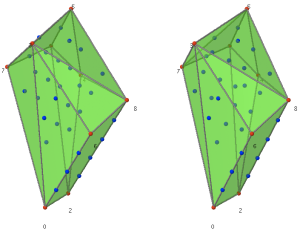
\includegraphics[width=8em]{polytope.png}

Folgen: \texttt{sloane\_find({\it Liste})}, \texttt{sloane.}$\langle$Tab$\rangle$  

Partitionen: \texttt{P=Partitions({\it n})}\quad \texttt{P.count()}

Kombinationen: \texttt{C=Combinations({\it Liste})}\quad\texttt{C.list()}

Kartesisches Produkt: \texttt{CartesianProduct(P,C)}

Tableau: \texttt{Tableau([[1,2,3],[4,5]])}

W�rter: \verb|W=Words("abc"); W("aabca")|

Teilgeordnete Mengen: \texttt{Poset([[1,2],[4],[3],[4],[]])}

Wurzelsysteme: \verb|RootSystem(["A",3])|

Kristalle: \verb|CrystalOfTableaux(["A",3], shape=[3,2])|

Verb�nde/Polytope: \verb|A=random_matrix(ZZ,3,6,x=7)|

\verb|L=LatticePolytope(A)    L.npoints()   L.plot3d()|

%*********************************************
\hr\textbf{Matrixalgebra}

$\begin{pmatrix}1\\2\end{pmatrix}=$ \verb|vector([1,2])|

$\begin{pmatrix}1&2\\3&4\end{pmatrix}=$ \verb|matrix(QQ,[[1,2],[3,4]], sparse=False)|

$\begin{pmatrix}1&2&3\\4&5&6\end{pmatrix}=$ \verb|matrix(QQ,2,3,[1,2,3, 4,5,6])|

$\left|\begin{matrix}1&2\\3&4\end{matrix}\right|=$
\verb|det(matrix(QQ,[[1,2],[3,4]]))|

$Av=$ \verb|A*v| \quad $A^{-1}=$ \verb|A^-1| \quad $A^t=$ \verb|A.transpose()|

L�se $Ax=v$: \verb| A\v  | oder \verb| A.solve_right(v)|

L�se $xA=v$: \verb| A.solve_left(v)|

reduzierte Stufenform: \verb| A.echelon_form()|

Rang und Defekt: \verb|A.rank()    A.nullity()|

Hessenberg-Form: \verb|A.hessenberg_form()|

Charakteristisches Polynom: \verb|A.charpoly()|

Eigenwerte: \verb|A.eigenvalues()| 

Eigenvektoren: \verb|A.eigenvectors_right()| (auch \verb|left|)

Gram-Schmidt-Orthogonalisierung: \verb|A.gram_schmidt()|

Zeichnen: \verb|A.plot()|

LLL Reduktion: \verb|matrix(ZZ,...).LLL()|

Hermite Normalform: \verb|matrix(ZZ,...).hermite_form()|

%*********************************************
\hr\textbf{Lineare Algebra}

\includegraphics[width=12em,height=6em]{linalg}

Vektorraum $K^n = $ \verb| K^n | e.g. \verb| QQ^3   RR^2   CC^4|

Unterraum: \verb|span(|{\it Vektoren, K�rper}\verb|)| 

Z.B., \verb|span([[1,2,3], [2,3,5]], QQ)|

Kern: \verb|A.right_kernel()| (auch \verb|left_kernel()|)

Vereinigung und Schnitt: \verb|U + V | and \verb| U.intersection(V)|

Basis: \verb|U.basis()|

Basismatrix: \verb|U.basis_matrix()|

Einschr�nkung auf den Unterraum: \texttt{A.restrict(U)}

Vektor in Basisdarstellung: \texttt{U.coordinates({\it Vektor})}

%*********************************************
\hr\textbf{Numerik}

Pakete: \verb|import numpy, scipy, cvxopt|

Minimalisierung: \verb|var("x y z")|

\verb|   minimize(x^2+x*y^3+(1-z)^2-1, [1,1,1])|


%*********************************************
\hr\textbf{Zahlentheorie}

Primzahlen: \verb|prime_range(n,m)|, \verb|is_prime|, \verb|next_prime|

Faktorisierung: \verb|factor(n)|, \verb|qsieve(n)|, \verb|ecm.factor(n)|

Kronecker Symbol: $\left(\frac{a}{b}\right) = $ \texttt{kronecker\_symbol({\it a},{\it b})}

Kettenbr�che: \verb|continued_fraction(x)|

Bernoulli-Zahlen: \texttt{bernoulli(n)}, \texttt{bernoulli\_mod\_p(p)}

Elliptische Kurven: \verb|EllipticCurve([|$a_1,a_2,a_3,a_4,a_6$\verb|])|

Dirichlet-Charaktere: \texttt{DirichletGroup({\it N})}

%Congruence subgroups: \texttt{Gamma0({\it N})}, \texttt{Gamma1({\it N})}, \texttt{GammaH}

Modulformen: \texttt{ModularForms({\it Level,Gewicht})}

Modulsymbole: \texttt{ModularSymbols({\it Level,Gewicht,Zeichen})}

Brandt Moduln: \texttt{BrandtModule({\it Level,Gewicht})}

Abelsche Variet�ten: \texttt{J0({\it N})}, \texttt{J1({\it N})}

%*********************************************
\hr\textbf{Gruppentheorie}

\texttt{G = PermutationGroup([[(1,2,3),(4,5)],[(3,4)]])}

\texttt{SymmetricGroup({\it n})}, \texttt{AlternatingGroup({\it n})} 

Abelsche Gruppen: \texttt{AbelianGroup([3,15])}

Matrixgruppen: \texttt{GL, SL, Sp, SU, GU, SO, GO}

Funktionen: \texttt{G.sylow\_subgroup(p)}, \texttt{G.character\_table()}, 

\texttt{G.normal\_subgroups()}, \texttt{G.cayley\_graph()}


%*********************************************
\hr\textbf{Nichtkommutative Ringe}

Quaternionen: \texttt{Q.<i,j,k> = QuaternionAlgebra(a,b)}

Freie Algebren: \texttt{R.<a,b,c> = FreeAlgebra(QQ, 3)}

%Steenrod algebra: \texttt{SteenrodAlgebra({\it prime})}

%*********************************************
\hr\textbf{Python Module}

\verb|import| \emph{Modul\_Name}

\verb|Modul_Name.|$\langle$Tab$\rangle$ und \verb|help(Modul_Name)|

%\verb|sage.|\emph{module\_name}\verb|.all.|$\langle$tab$\rangle$ shows exported commands

%\mbox{Std packages: Maxima GP/PARI GAP Singular R Shell ...}

%Opt packages: Biopython Gnuplot Kash ...

%\%\emph{package\_name} then use package command syntax

%*********************************************
\hr\textbf{Laufzeitanalyse}

\verb|time| \emph{befehl}: \quad  Zeigt Laufzeitinformationen

\verb|timeit("|\emph{befehl}\verb|")|: genaue Zeitmessung von {\it befehl}

\verb|t = cputime(); cputime(t)|: vergangene CPU Zeit

\verb|t = walltime(); walltime(t)|: vergangene Echtzeit

\verb|%pdb|: Interaktiven Debugger anschalten (Kommandozeile)

\verb|%prun |\emph{befehl}: Analysiere \emph{befehl} (Kommandozeile)

\end{multicols*}

\end{document}
